\chapter{Observatorio Pierre Auger}
\label{ch:detectorAuger}

El objetivo del Observatorio Pierre Auger es colectar eventos de rayos c\'osmicos con energ\'ias mayores a $10^{18}\ eV$, con el fin de comprender su naturaleza. Entre otras cosas, se busca reconstruir el espectro energ\'etico con precisi\'on sin precedentes, medir las direcciones de arribo y estudiar la composici\'on de los mismos.
Para alcanzar esta meta, se decidi\'o construir dos detectores h\'ibridos, uno en el hemisferio Sur y otro en el Norte.

El Observatorio Sur se encuentra en Pampa Amarilla a una altitud promedio de $\sim 1400\ m$, cerca de Malarg\"ue, en la provincia de Mendoza, Argentina.
\'Este lugar fue elegido debido a que el terreno es relativamente plano, variando menos de $200\ m$ en toda la extensi\'on del observatorio, y el clima \'arido con cielos despejados, condiciones ideales para un detector h\'ibrido de este tipo.

	\section{Detector H\'ibrido}
	Este detector combina las fortalezas de dos t\'ecnicas de detecci\'on: una grilla triangular de 1600 detectores Cherenkov (detector de superficie o SD) y 4 detectores de fluorescencia (detector de fluorecencia o FD).
	El detector h\'ibrido tiene importantes ventajas sobre cada una de las t\'ecnicas operando por separado, ya que observar lluvias en simult\'aneo permite identificar las fuentes de incertezas sistem\'aticas de cada t\'ecnica y medir independientemente propiedades de la lluvia.
	Las ventajas principales del detector de superficie son que puede operar el $100 \%$ del tiempo, su respuesta es poco dependiente del clima, su apertura se encuentra bien definida y es independiente de la energ\'ia por encima de $10^{19}\ eV$, su se\~nal puede autocalibrarse usando muones de rayos c\'osmicos  y tiene una alta sensitividad a lluvias que lleguen con grandes \'angulos cenitales. 
	Pero un experimento que s\'olo conste de un SD no podr\'ia realizar una reconstrucci\'on en energ\'ia sin asumir qu\'e part\'icula inici\'o la lluvia y una simulaci\'on de por medio~\cite{busca_thesis}.
	Por otro lado, el detector de fluorescencia posee la ventaja de medir directamente el perfil longitudinal de las EAS y poder realizar una medici\'on calorim\'etrica de la energ\'ia, sin necesidad de simulaciones. Pero la desventaja de este detector es que s\'olo puede realizar mediciones en noches sin luna y sin nubes, aproximadamente un $10 - 15 \%$ del tiempo de medici\'on.
	
	Al combinar ambas t\'ecnicas de medici\'on, es posible realizar una calibraci\'on cruzada entre ambos detectores, que permite calibrar en energ\'ia el SD sin ninguna suposici\'on sobre la part\'icula incidente.
	De hecho, se observa una correlaci\'on entre el tama\~no de la lluvia en el SD y la energ\'ia reconstruida con el FD.
	Al mismo tiempo, los eventos observados por ambos detectores tienen una mejora significativa en la reconstrucci\'on de la geometr\'ia de la lluvia y la energ\'ia de la misma.
	
	En la figura \ref{fig:plano_auger} se observa la disposici\'on geom\'etrica del detector.
	Los puntos negros corresponden a los detectores Cherenkov, separados por $1.5\ km$ en un arreglo triangular.
	Tambi\'en se observan los 4 detectores de fluorecencia, cada uno con 6 telescopios, cuya direcci\'on de observaci\'on se denota con lineas negras.
	
	\begin{figure}[h!]
		\begin{center}
		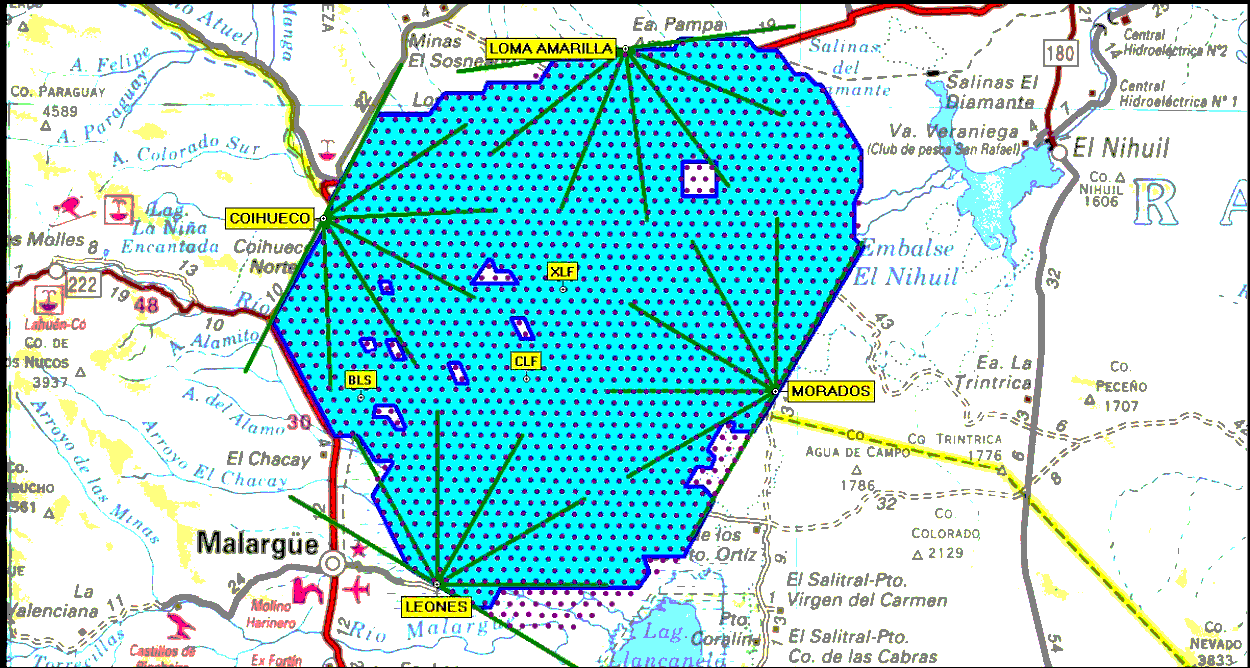
\includegraphics[width=\textwidth]{fig/detectorAuger/array}
		\caption{\label{fig:plano_auger} Ubicaci\'on geogr\'afica del Observatorio Pierre Auger. Los puntos negros dentro del \'area turquesa representan los tanques en funcionamiento a finales de 2009. 
		Las l\'ineas verdes indican el campo de visi\'on de cada uno de los 6 telescopios de cada detector de fluorecencia.}
		\end{center}
	\end{figure}
	
	Los eventos registrados se clasifican de la siguiente manera:
	\begin{itemize}
		\item Eventos SD: s\'olo detectados por la grilla de superficie.
		\item Eventos FD:
		\begin{itemize}
			\item Mono: s\'olo un detector de fluorescencia lo observa
			\item Stereo: lo observan 2 o m\'as detectores de fluorescencia 
		\end{itemize} 
		\item Eventos H\'ibridos:
		\begin{itemize}
			\item Simple: 1 detector FD + 1 tanque SD o algunos tanques SD, pero no suficientes como para hacer una reconstrucci\'on independiente SD.
			\item Dorados: 1 detector FD + $n$tanques SD, con $n$ suficientemente grande como para hacer una reconstrucci\'on SD independiente.
			\item Platino: 2 o m\'as detectores FD + cualquier informaci\'on del SD.
		\end{itemize}
	\end{itemize}
	
	\section{Detector de superficie}
	
	El detector de superficie del Observatorio Pierre Auger consta de 1600 tanques Cherenkov ubicados en un arreglo hexagonal, en el que cada tanque se encuentra a $1.5\ km$ de sus 6 vecinos, cubriendo en total una superficie de $3000\ km^2$.
	
	El objetivo de cada unidad del detector es colectar la radiaci\'on Cherenkov emitida por las part\'iculas que pasan por su interior.
	Cada una consiste de un tanque cil\'indrico de polietileno de $3.6\ m$ de di\'ametro y $1.55\ m$ de alto, cubriendo un {\em liner} repleto de 12 toneladas de agua excepcionalmente pura. 
	El {\em liner} es un bolsa pl\'astica cil\'indrica de $1.2\ m$ de altura, que es negra por fuera para sellarla de luz externa mientras que dentro est\'a protegida con Tyvek para reflejar la luz Cherenkov. 
	La luz Cherenkov es colectada por tres fototubos de 8 pulgadas cada uno, y su señal es continuamente registrada por un convertidor anal\'ogico digital (FADC) en bines de $25\ ns$.
	Esta se\~nal es muestreada con una frecuencia de $40\rm \ MHz$ y una resoluci\'on de 10 bits mediante un CPU, que tambi\'en realiza las primeras decisiones de trigger.
	Cada estaci\'on est\'a equipada, adem\'as, con un GPS que permite sincronizar los relojes de todas las estaciones con una precisi\'on de $8\rm \,ns$ \cite{auger_prop04}.
	En la figura \ref{fig:tanque} se muestra una foto de un tanque ya instalado seguido de un esquema que especifica cada una de sus partes.
	
	Puesto que muchas veces la zona donde se encuentra el tanque es de dif\'icil acceso, \'estos fueron diseñados para ser unidades aut\'onomas equipadas con un panel solar, bater\'ias y una antena de comunicaci\'on.
	Las trazas de los fototubos y los datos de tiempo son almacenados por la estaci\'on en un buffer que es posteriormente transmitido a una computadora central en el centro de adquisici\'on de datos (CDAS).
	
	\begin{figure}[h!]
		\begin{center}
		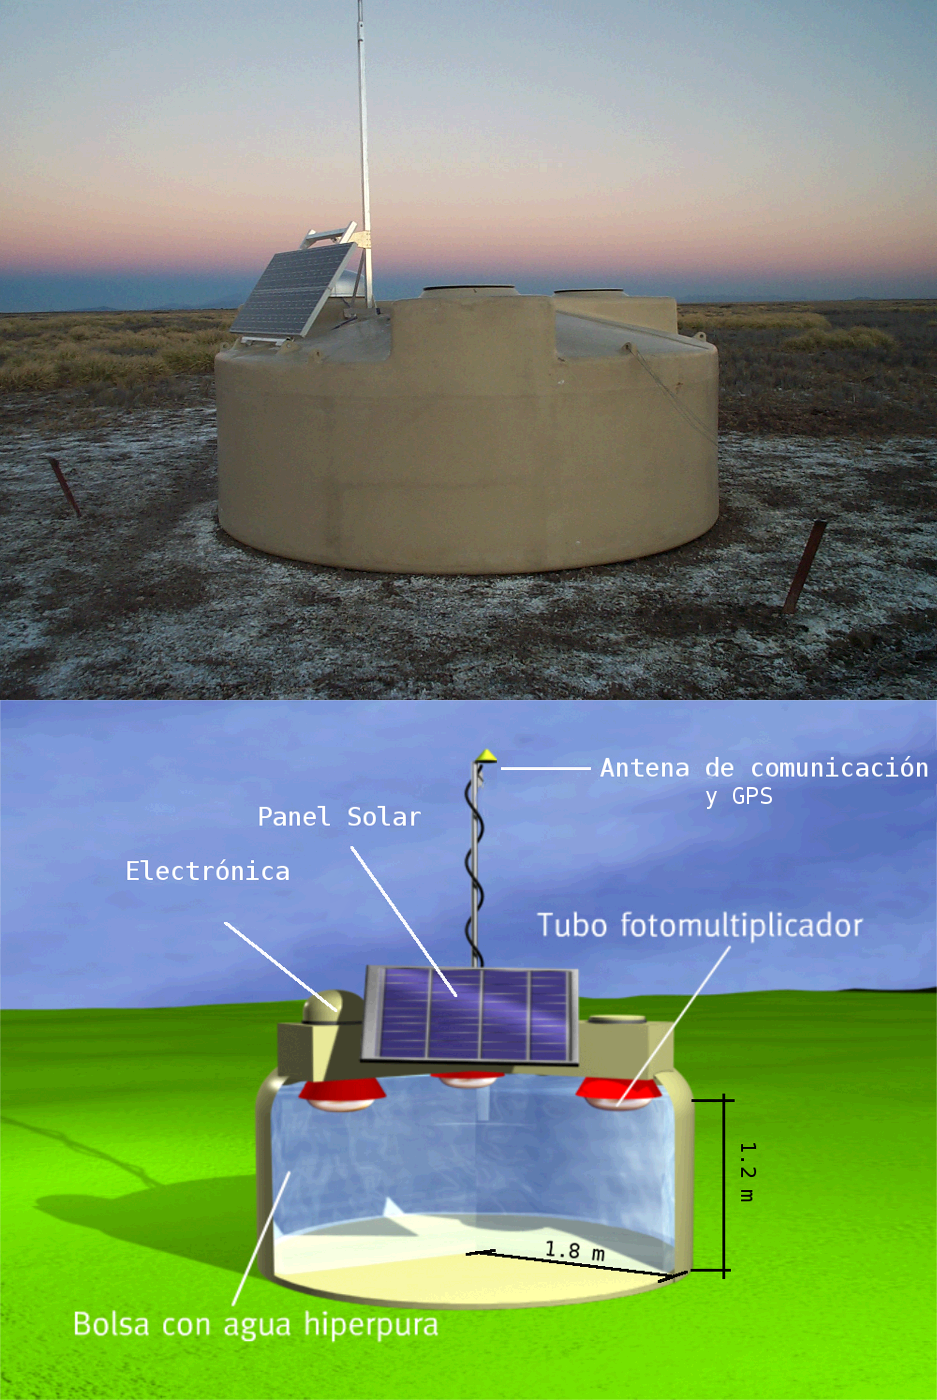
\includegraphics[width=0.7\textwidth]{fig/detectorAuger/Tanque00}
		\caption{\label{fig:tanque} En la parte superior (inferior) de la figura se muestra una foto (esquema) de uno de los tanques del arreglo de superficie del Observatorio Pierre Auger, en Malarg\"ue.}
		\end{center}
	\end{figure}

		\subsection{Calibraci\'on del detector de superficie}
		
		La Colaboraci\'on Auger ha adoptado al VEM (Vertical Equivalent Muon) como unidad de medida para las señales adquiridas por el SD.
		El VEM se define como la señal promedio producida en un tanque del SD al ser atravesado por su eje por un mu\'on vertical.
		
		Dada la gran cantidad de estaciones y la dificultad de acceder a ellas, el proceso de calibraci\'on implementado en el SD es realizado de manera aut\'onoma por la computadora de cada tanque. 
		Los muones atmosf\'ericos tienen una frecuencia de arribo uniforme sobre todo el detector lo que los hace ideales para lograr una buena calibraci\'on relativa entre los tanques. 
		Es por ello que el algoritmo de calibraci\'on implementado se basa en la medici\'on de su espectro. 
		La figura \ref{Calibracion_Muones} muestra un espectro t\'ipico adquirido por uno de los tanques. 
		A partir de experiencias realizadas utilizando un tanque en conjunci\'on con un telescopio de muones se ha determinado que el segundo\footnote{El primero es un artefacto} pico corresponde a \cant{1.05}{VEM}. 
		Utilizando esta referencia cada tanque ajusta su ganancia de manera tal que coincida con la de los dem\'as.
		
		\begin{figure}[ht]
			\begin{center}
			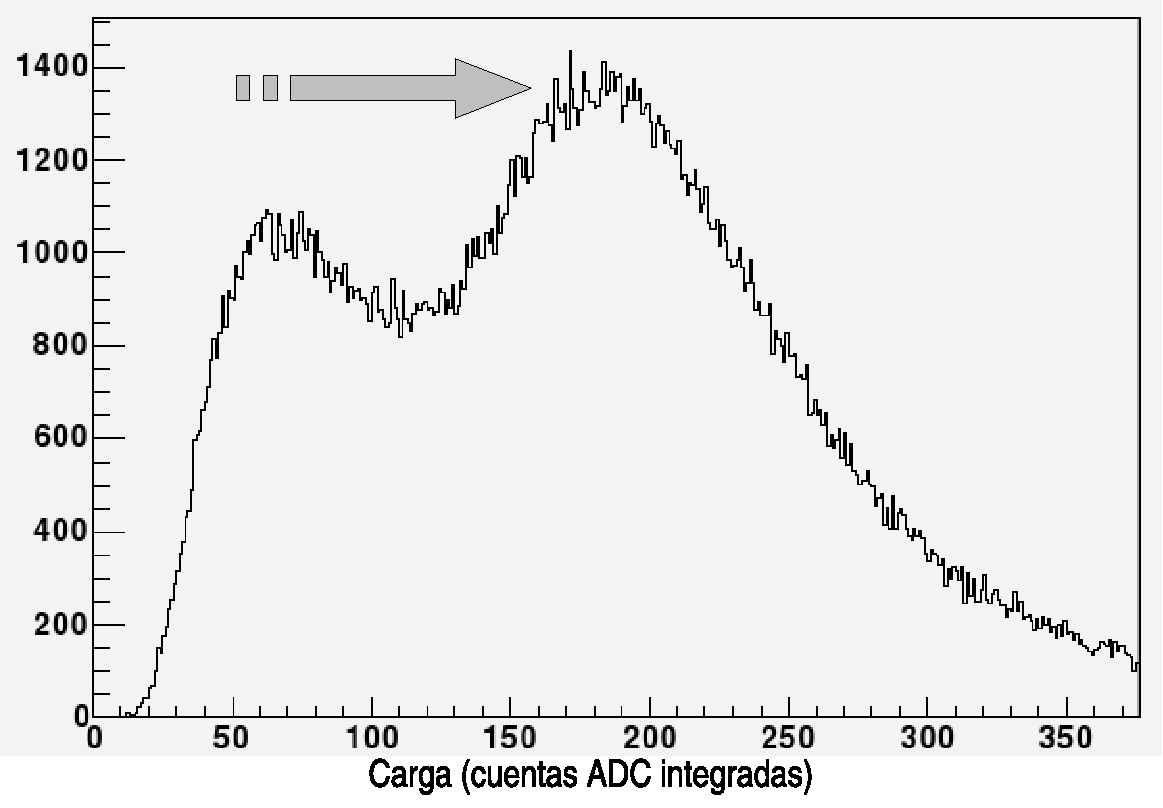
\includegraphics[width=0.8\textwidth]{fig/detectorAuger/vem}
			\caption{Espectro de muones atmosf\'ericos para una coincidencia de tres fototubos. El pico se\~nalado corresponde a \cant{1.05}{VEM}}
			\label{Calibracion_Muones}
			\end{center}
		\end{figure}
		
		
		\subsection{Niveles de trigger}
		\label{sbsc:trig_levels}
		
		Con el fin de limitar la cantidad de eventos almacenados y minimizar la contaminaci\'on, el Proyecto Auger ha adoptado una estructura jer\'arquica de disparos para el detector de superficie, que puede clasificarse b\'asicamente en dos niveles \cite{icrctri}:
		
		\begin{shortitemize}
		\item Trigger de bajo nivel
		\item Trigger de alto nivel
		\end{shortitemize}
		
			\subsubsection{Trigger de bajo nivel}
			
			Este nivel de trigger se aplica en tiempo real en cada estaci\'on con dos fines, disminuir la frecuencia de detecci\'on de muones atmosf\'ericos y distinguir entre las componentes mu\'onicas y electromagn\'eticas de la lluvia.
			Aqu\'i la nomenclatura utilizada \cite{nimtrig}:
			
			\begin{itemize}
			\item T1-Threshold (T1-TH): Corresponde a una traza que supera \cant{1.75}{VEM} en los tres PMT's del taque. El objetivo principal de este criterio es disminuir de \cant{\approx3}{kHz} a \cant{\approx 100}{Hz} la detecci\'on de muones atmosf\'ericos.
			\item T1-Time Over Threshold (T1-ToT): Corresponde a una se\~nal que supera \cant{0.2}{VEM} en m\'as de 13 bines de FADC dentro de una ventana de 120 bines (\cant{3}{\mu s}), para dos cualesquiera de los 3 PMT's. Este criterio busca detectar lluvias con gran componente electromagn\'etica al nivel del suelo y la parte mas alejada de las lluvias verticales, debido a que la dispersi\'on temporal en el arribo de las part\'iculas al detector es grande (\cant{\approx 300}{ns} para un tanque que se encuentra a \cant{1000}{m} del eje en una lluvia vertical \cite{disp1,disp2}). La frecuencia de disparo de este nivel es \cant{\approx 1.6}{Hz}.
			\item T2-Threshold (T2-TH): Para cumplir esta categor\'ia se pide una traza que supere \cant{3.2}{VEM}. Este criterio baja la frecuencia de disparo de \cant{\approx 100}{Hz} a \cant{\approx 20}{Hz}.
			\item T2-Time Over Threshols (T2-ToT): Todos los T1-ToT pasan directamente a esta categor\'ia. %La frecuencia de aparicion de este tipo de disparo es \cant{\approx 1.6}{Hz}
			\end{itemize}
			
			En las figuras \ref{fig:t2_th} y \ref{fig:t2_tot} se muestran las trazas de los tres PMT's para eventos clasificados como T2-TH y T2-ToT respectivamente.
			
			\begin{figure}[h!]
				\begin{center}
				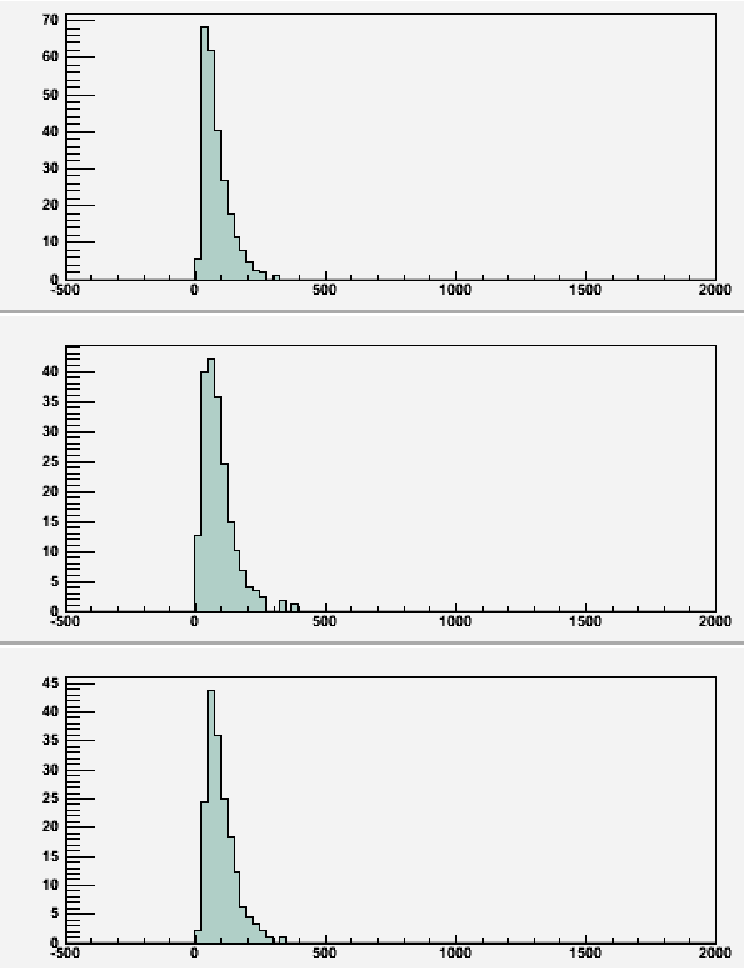
\includegraphics[width=0.45\textwidth]{fig/detectorAuger/Threshold}
				\caption{\label{fig:t2_th} Ejemplo de traza que produce un T2-Threshold.}
				\end{center}
			\end{figure}
			\begin{figure}[h!]
				\begin{center}
				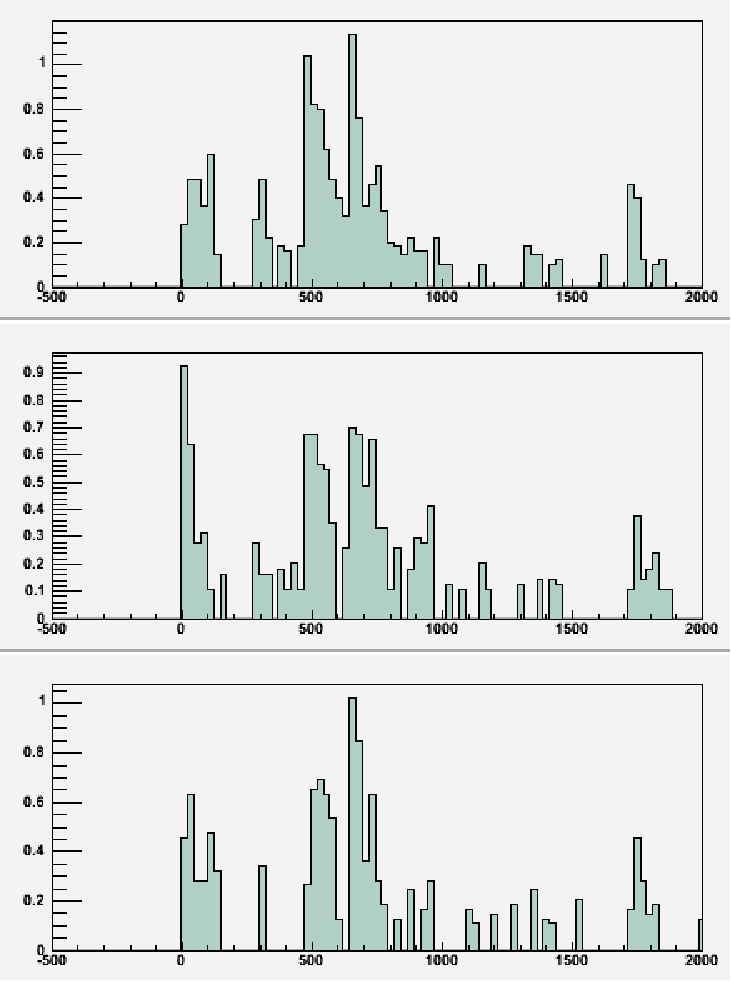
\includegraphics[width=0.45\textwidth]{fig/detectorAuger/ToT}
				\caption{\label{fig:t2_tot} Ejemplo de traza que produce un T2-ToT}
				\end{center}
			\end{figure}
			
			Todas las estaciones con T1 o T2 se guardan durante \cant{10}{s} esperando un posible trigger de m\'as alto nivel, T3.
			
			\subsubsection*{Trigger de alto nivel}
			
			\titulo{Trigger del detector T3} El siguiente nivel de trigger es T3, que es iniciado desde el CDAS seg\'un cierta combinaci\'on espacial y temporal de estaciones con T2.
			Una vez detectado un T3, son guardadas las trazas de todas las estaciones con T1 o T2 dentro de una ventana temporal de \cant{30}{\mu s}.
			El trigger del detector se realiza seg\'un dos categorias:
			
			\begin{itemize}
			\item 3ToT ($\rm ToT2C_1\&3C_2$): Este criterio requiere que al menos 3 detectores sean ToT. Tambi\'en requiere cierta compacticidad en la distribuci\'on espacial de la se\~nal, pidiendo que al menos dos tanques sean primeros vecinos y el tercero se encuentre en la segunda corona de alguno de los dos. La nomenclatura de esta categor\'ia es $\rm ToT2C_1\&3C_2$, donde $\rm C_n$ se refiere a la corona n-\'esima desde alguno de los tanques, siempre el mismo. En el panel izquierdo de la figura \ref{fig:coronas} se muestra una configuraci\'on de tanques que cumple con esta categor\'ia. Una vez satisfecho el criterio espacial, se somete la configuraci\'on a un criterio temporal, pidiendo que cada tanque se encuentre separado a menos de \cant{(6+5{\rm C_n})}{ns} del primero, donde $C_n$ indica en n\'umero de corona en el que se encuentra. Se registran del orden de 1600 de estos eventos por d\'ia, siendo el \cant{90}{\%} de estos eventos f\'isicos, debido al bajo nivel de contaminaci\'on que presentan los tanques con T2-ToT. El \cant{10}{\%} restante se debe al permisivo criterio temporal.
			\item 4 fold T2 ($\rm2C_1\&3C_2\&4C_4$): Este criterio es mucho menos exigente, pidiendo cuatro T2 con una compacticidad espacial moderada. Para satisfacer esta categor\'ia se pide que dos tanques sean primeros vecinos, que el tercero se encuentre dentro de la segunda corona de alguno de los dos y que exista al menos un tanque m\'as en la cuarta corona del anterior. Un ejemplo de esta distribuci\'on espacial se muestra en el panel derecho de la figura \ref{fig:coronas}. Tambi\'en se pide el mismo criterio temporal que para la categor\'ia $\rm ToT2C_1\&3C_2$. Este nivel de trigger tiene buena eficiencia para eventos inclinados, pero es muy sensible a disparos casuales de los tanques, por lo que de los 1200 eventos registrados diariamente, \cant{\approx 10}{\%} de ellos corresponden a lluvias reales.
			\end{itemize}
			
			\begin{figure}[h!]
				\begin{center}
				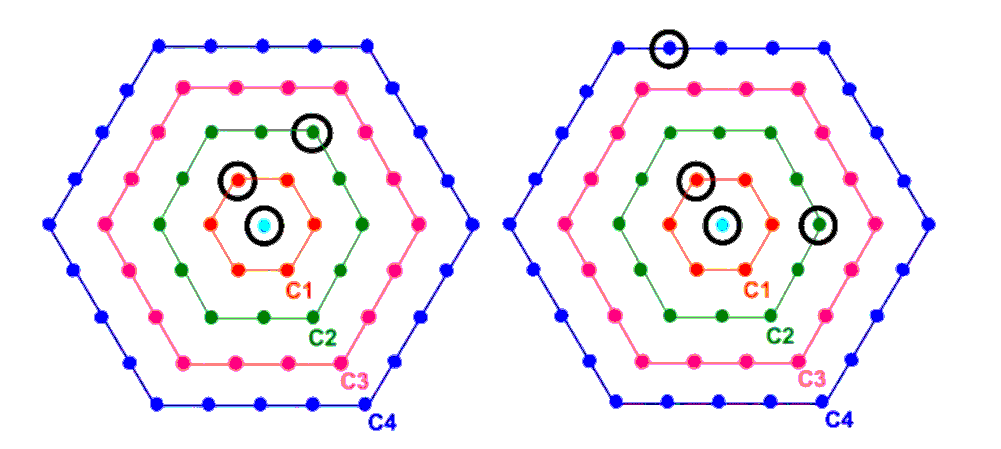
\includegraphics[width=\textwidth]{fig/detectorAuger/coronas}
				\caption{\label{fig:coronas} Ejemplos de configuraciones T3: en el panel izquierdo (derecho) se muestra un ejemplo una configuraci\'on que satisface el criterio $\rm ToT2C_1\&3C_2$ ($\rm 2C_1\&3C_4\&4C_4$). $\rm C_1$, $\rm C_2$, $\rm C_3$ y $\rm C_4$ indican la primera, segunda, tercera y cuarta corona de vecinos respectivamente, a 1.5, 3, 4.5 y 6 km para un dado detector.}
				\end{center}
			\end{figure}
			
			En la figura \ref{fig:diagtrig} se muestra la jerarqu\'ia de triggers hasta T3.
			\vspace{0.5cm}
			
			\begin{figure}[h!]
				\begin{center}
				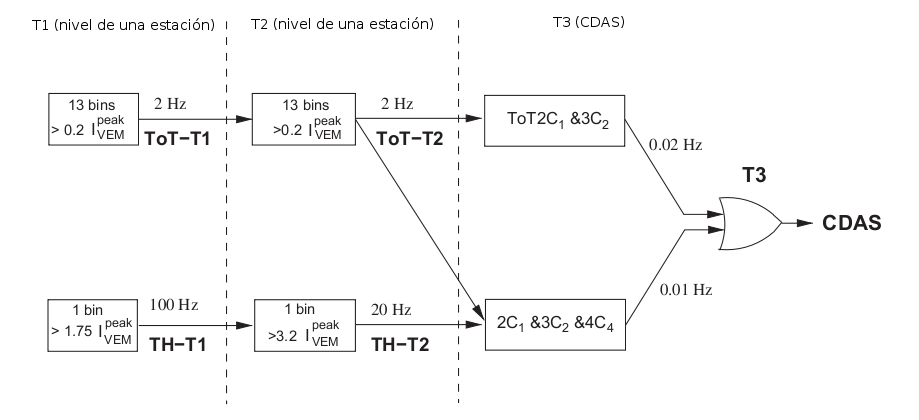
\includegraphics[width=0.9\textwidth]{fig/detectorAuger/Trigger_2}
				\caption{\label{fig:diagtrig} Jerarqu\'ia de trigger hasta T3.}
				\end{center}
			\end{figure}
			
			\titulo{Trigger f\'isico T4} Este nivel de trigger se aplica para remover lso eventos que dieron T3 debido a disparos casuales de los tanques.
			Con este fin, se clasifican los eventos en dos nuevas categor\'ias:
			
			\begin{itemize}
			\item 3-ToT: Para cumplir con esta categor\'ia se deben encontrar tres tanques T2-ToT en la primer corona de alguno de los tres y formando un tri\'angulo. Los tanques deben estar alejados como m\'aximo \cant{2700}{m}. Tambi\'en se pide que el tiempo de disparos de las estaciones entre si sea compatible con un frente que se mueve a la velocidad de la luz. Esta categor\'ia es muy eficiente filtrando eventos casuales, m\'as aun si la direcci\'on de arribo de la lluvia es $<60º$ (\cant{98}{\%} de eficiencia en estas condiciones). Los eventos accidentales que pasan esta categor\'ia son menos que uno por d\'ia.
			\item $\rm 4C_1$: Este criterio requiere cuatro estaciones dentro de la primer corona de alguno de los tanques, todas con cualquier T2. Tambi\'en se pide que los tiempos de arribo sean compatibles con un frente que se mueve a la velocidad de la luz. La frecuencia con la que se da este trigger es \cant{\approx 0.001}{Hz} y la eficiencia para lluvias de $<60º$ es \cant{\approx 100}{\%}.
			\end{itemize}
			\vspace{0.5cm}
			
			\titulo{Trigger de calidad T5} Esta categor\'ia se define para filtrar lluvias incompletas debido a que fueron detectadas en el borde del detector o en alg\'un agujero debido a estaciones fuera de servicio al momento de arribo.
			De esta manera se busca evitar errores al momento de la reconstrucci\'on debido a que tal vez la parte m\'as importante de la lluvia no fue detectada.
			Se definen las dos siguientes categor\'ias:
			
			\begin{itemize}
			\item T5: Esta categor\'ia requiere que la estaci\'on con mayor se\~nal integrada se encuentre rodeada de seis estaciones activas.
			\item ICRC T5: Igual que T5, pero este requiere s\'olo 5 de las 6 estaciones y que el n\'ucleo reconstruido de la lluvia se encuentre dentro de un tri\'angulo formado por tres estaciones activas.
			\end{itemize}
			
			En la figura \ref{fig:diagtrig2} se muestra la jerarqu\'ia de triggers desde T3.
			
			\begin{figure}[h!]
				\begin{center}
				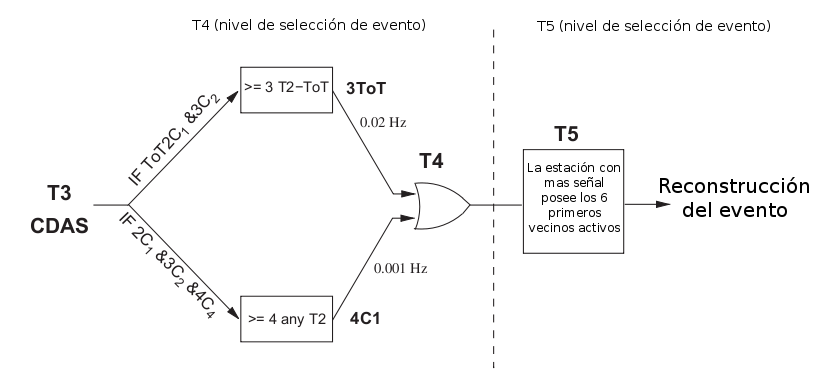
\includegraphics[width=0.9\textwidth]{fig/detectorAuger/Trigger_3}
				\caption{\label{fig:diagtrig2} Jerarqu\'ia de trigger desde T3.}
				\end{center}
			\end{figure}
